Thay vì chỉ kiểm soát phương sai như phương pháp Markowitz truyền thống, nghiên cứu thiết lập bài toán tối ưu hóa phi tuyến (SLSQP) trên 10.000 kịch bản vừa tạo ra. Mục tiêu cốt lõi là cực tiểu hóa rủi ro đuôi, đại diện bởi chỉ số Giá trị chịu rủi ro có điều kiện (CVaR) tại mức ý nghĩa $\alpha = 95\%$.

\begin{figure}[H]
    \centering
    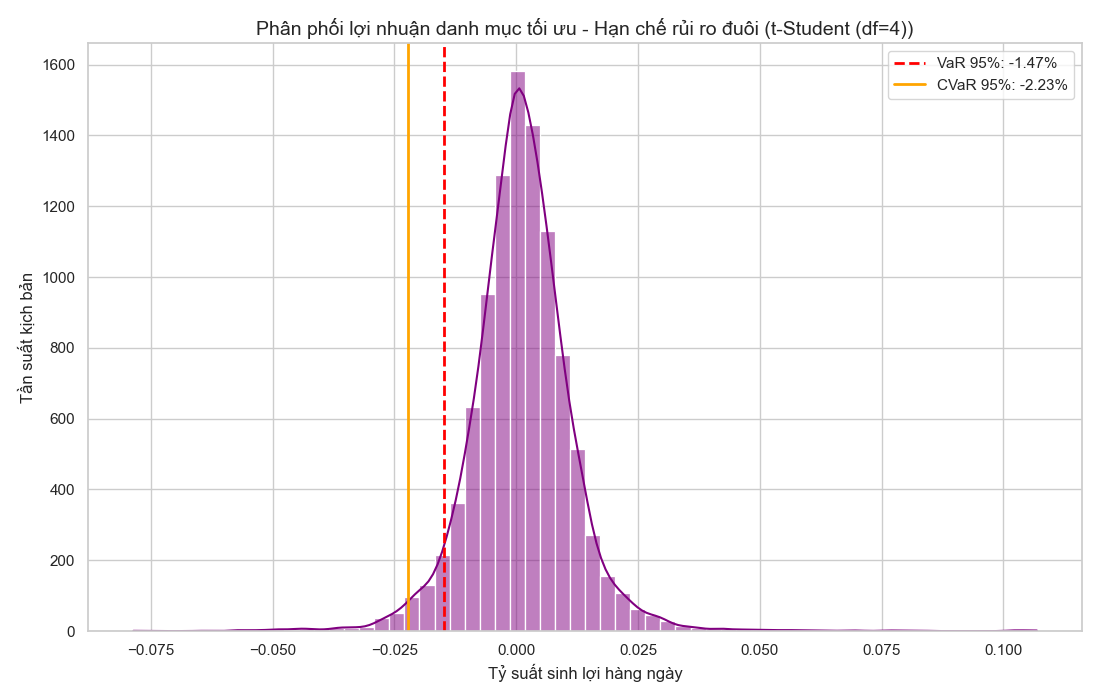
\includegraphics[width=0.85\textwidth]{optimal_cvar_portfolio.png}
    \caption{Phân phối lợi suất của danh mục tối ưu t-Student Copula và các ngưỡng rủi ro}
    \label{fig:cvar_distribution}
\end{figure}

\begin{flushleft}
\textbf{Nhận xét:}
\begin{itemize}
    \item Quan sát Hình \ref{fig:cvar_distribution}, hai đường ranh giới quan trọng được xác định bao gồm VaR (màu đỏ) đại diện cho ngưỡng tổn thất tối đa ở điều kiện bình thường và CVaR (màu cam) đại diện cho thiệt hại trung bình khi thị trường rơi vào trạng thái cực đoan.
    \item Việc áp dụng thuật toán tối ưu hóa CVaR đã giúp thu hẹp đáng kể rủi ro của danh mục. Cụ thể, ngưỡng tổn thất tối đa (VaR 95\%) đã được cải thiện tích cực từ mức -1.56\% (trước tối ưu ở Hình \ref{fig:daily_return_dist}) xuống chỉ còn -1.47\% (sau tối ưu ở Hình \ref{fig:cvar_distribution}).
    \item Sự chênh lệch này minh chứng rõ nét cho hiệu quả thực chứng của thuật toán trong việc cấu trúc lại tỷ trọng tài sản. So với danh mục Markowitz truyền thống vốn dễ vỡ trước các đợt bán tháo đồng loạt, danh mục Copula-CVaR đã chủ động thiết lập một lớp phòng vệ an toàn và tối ưu hơn hẳn cho nhà đầu tư.
\end{itemize}
\end{flushleft}
